% !TeX spellcheck = pl_PL
\documentclass[10pt,a4paper]{article}

\usepackage{geometry}
\geometry{
	a4paper,
	total={170mm,257mm},
	left=20mm,
	top=20mm,
}


% większość można wywalić, przekopiowane z projektu z MNUMów
\usepackage{mathtools}
\usepackage{polski}
\usepackage{amsfonts}
\usepackage{amsmath}
\usepackage[T1]{fontenc}
\usepackage{listings}
\usepackage{booktabs}
\usepackage{csvsimple}
\usepackage{geometry}
\usepackage{siunitx}
\usepackage{caption}
\usepackage{booktabs}
\usepackage{longtable}
\usepackage{float}
\usepackage{algpseudocode}
\usepackage{algorithm}
\usepackage{csquotes}
\usepackage{hyperref}
\usepackage{graphicx}
\usepackage{subcaption}


\captionsetup[table]{skip=10pt}

\sisetup{round-mode=places, round-precision=3, round-integer-to-decimal, scientific-notation = true, table-format = 1.3e2, table-number-alignment=center, group-separator={,}}


\title{Inżynieria Uczenia Maszynowego - projekt (etap 2)}
\author{Tomasz Owienko \and Anna Schäfer}
\date{10.01.2024}


% definicja problemu biznesowego
% zadania modelowania
% założenia
% kryteria sukcesu
% analiza danych z perspektywy realizacji zadań


\begin{document}
\maketitle

\section{Temat projektu}




Temat projektu przekazany przez Klienta:

\begin{displayquote}
	\textit{Może bylibyśmy w stanie wygenerować playlistę, która spodoba się kilku wybranym osobom jednocześnie? Coraz więcej osób używa Pozytywki podczas różnego rodzaju imprez i taka funkcjonalność byłaby hitem!}
\end{displayquote}


\section{Modele}


\subsection*{Model bazowy}
Model bazowy został zaimplementowany jako prosty algorytm losujący utwory z historii odtwarzania poszczególnych użytkowników biorących udział w tworzeniu playlisty. Jest to podejście referencyjne, które posłuży do porównania z modelem zaawansowanym.

\subsection*{Model zaawansowany}
  Rozwiązanie opiera się na generowaniu rekomendacji dla pojedynczych użytkowników za pomocą modelu \href{https://arxiv.org/pdf/1507.08439.pdf}{LightFM}, a następnie łączeniu ich w docelową playlistę. Do playlisty wybierane jest $N$ utworów, które osiągnęły najwyższą średnią rangę w rekomendacjach poszczególnych użytkowników.

\subsection*{Selekcja/ocena istotności atrybutów}

Proces selekcji atrybutów został opisany w dokumentacji etapu pierwszego projektu. Ostatecznie wykorzystano następujące zestawy danych i atrybuty:
 
\begin{itemize}
\item \texttt{users.jsonl}
    \subitem Zdecydowano się na wykorzystanie jedynie informacji o \texttt{id} użytkownika
\item \texttt{sessions.jsonl}
    \subitem Nie odrzucono wstępnie żadnych atrybutów.
\item \texttt{tracks.jsonl}
    \subitem Odrzucono (na potrzeby modelowania) jedynie atrybut \texttt{name} - ponieważ pozostałe atrybuty nie są wykorzystywane w sposób bezpośredni, a jedynie służą do wygenerowania reprezentacji utworu w przestrzeni embeddingów, zdecydowano się nie odrzucać żadnego z nich.
\end{itemize}

Zamodelowano interakcje jako niejawne:
\begin{itemize}
    \item \texttt{action==like} $\Rightarrow$ 1
    \item \texttt{action!=like} $\Rightarrow$ 0.
\end{itemize}

Ponadto, ustandaryzowano wszystkie atrybuty numeryczne utworów.

\subsection*{Analityczne kryterium sukcesu}

Wyznaczanie rekomendacji dla pojedynczego użytkownika - pole pod krzywą ROC powyżej $0,6$ przy szacowaniu oceny dla utworów ze zbioru testowego (kryterium bezpośrednio związane z modelem).

Wyznaczanie rekomendacji dla wielu ($n$) użytkowników - model zaawansowany lepszy niż model bazowy. Jakość wyników mierzona będzie jako stopień klasteryzacji reprezentacji utworów wchodzących w skład playlisty. Stopień klasteryzacji określony będzie jako średnia odległość reprezentacji utworów od środka klastra w przestrzeni embeddingów modelu LightFM - jest ona generowana podczas trenowania modelu. Rekomendacje lepszego modelu powinny cechować się lepszą klasteryzacją, zatem średnia odległość powinna być niższa. Stopień klasteryzacji można potraktować jako minimalizowaną zmienną celu.

\subsection*{Strojenie hiperparametrów}

Model trenowanie modelu wymaga podania hiperparametrów:
\begin{itemize}
    \item \texttt{learning\_rate}
    \item \texttt{item\_alpha} - mnożnik współczynnika kary przy znajdowaniu embeddingów
    \item \texttt{no\_components} - rozmiar wektora reprezentującego utwór w przestrzeni embeddingów
\end{itemize}

Przetestowano około 550 kombinacji hiperparametrów dobieranych metodą losową z przedziałów:
\begin{itemize}
    \item \texttt{learning\_rate} $\in <10^{-5}, 10^{-0.7}>$
    \item \texttt{item\_alpha} $\in <10^{-6}, 10^{1}>$
    \item \texttt{no\_components} $\in <50, 80>$.
\end{itemize}

Wyniki oceniono pod kątem wpływu na pole pod krzywą ROC i stosunek średniej odległości od środka klastra poleconych utworów w modelu bazowym do tej samej miary w modelu zaawansowanym. Przy ocenianiu klasteryzacji uśredniano wyniki z 400 wygenerowanych playlist długości 20 dla losowej liczby użytkowników z przedziału $<2, 10>$. Przyjęto czas trenowania jako \texttt{epochs=10}. Zbiór danych podzielono na trenujący i testowy w stosunku $80/20$ wybierając losowe interakcje między użytkownikami a utworami, ustalono ziarno losowe modelu na \texttt{np.random.RandomState(12345678)}.


\begin{figure}[H]
\centering
\begin{subfigure}{.5\linewidth}
    \centering
    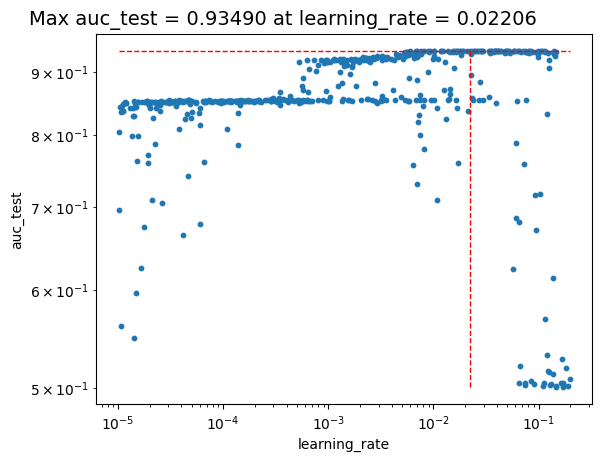
\includegraphics[width=1\linewidth]{image_2024-01-19_194944584.png}
\end{subfigure}%
\begin{subfigure}{.5\linewidth}
    \centering
    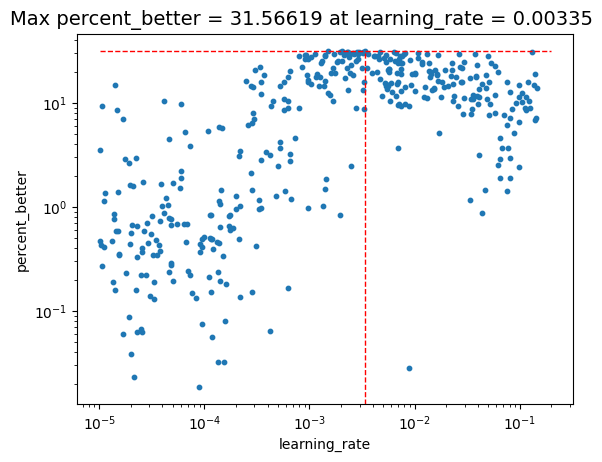
\includegraphics[width=1\linewidth]{image_2024-01-19_235211423.png}
\end{subfigure}
\begin{subfigure}{.5\textwidth}
    \centering
    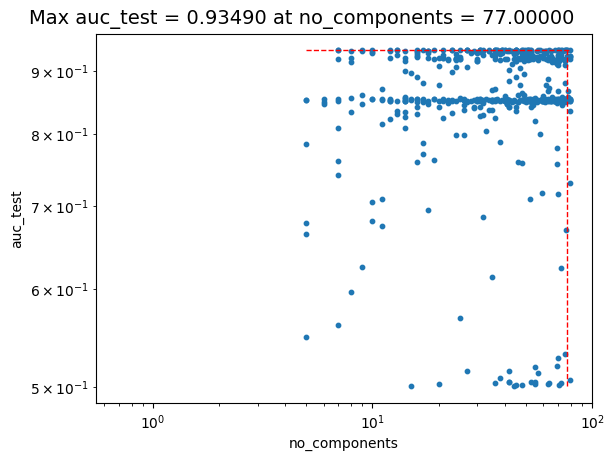
\includegraphics[width=1\linewidth]{image_2024-01-19_195516476.png}
\end{subfigure}%
\begin{subfigure}{.5\textwidth}
    \centering
    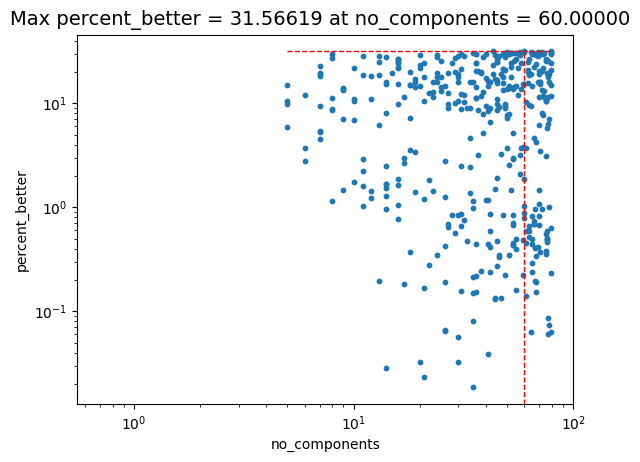
\includegraphics[width=1\linewidth]{image_2024-01-19_235314759.png}
\end{subfigure}
\begin{subfigure}{.5\textwidth}
    \centering
    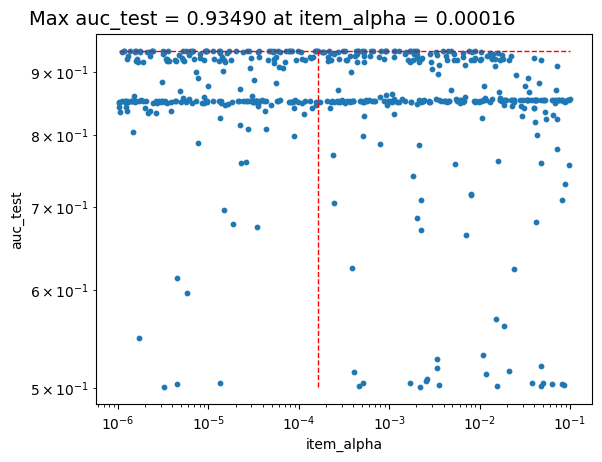
\includegraphics[width=1\linewidth]{image_2024-01-19_195441467.png}
\end{subfigure}%
\begin{subfigure}{.5\textwidth}
    \centering
    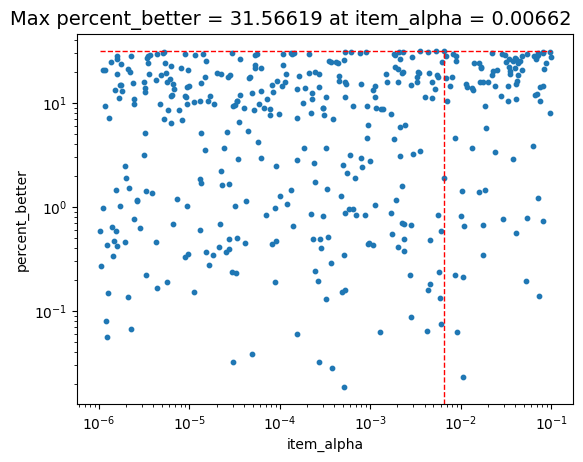
\includegraphics[width=1\linewidth]{image_2024-01-19_235352943.png}
\end{subfigure}
\caption[short]{Wpływ hiperparametrów na jakość modelu}
\end{figure}

Zebrano też uśrednione wyniki z 20 najlepszych kombinacji hiperparametrów dla miary ROC AUC i relatywnej jakości klasteryzacji:


\begin{center}
\begin{table}[H]
\centering
\begin{tabular}{lrr}
\toprule
 & mean & std \\
\midrule
learning\_rate & 0.032449 & 0.026287 \\
item\_alpha & 0.000542 & 0.000971 \\
no\_components & 41.700000 & 20.110484 \\
\hline
auc\_test & 0.934851 & 0.000019 \\
clustering\_fm & 0.551869 & 0.169077 \\
clustering\_base & 0.901284 & 0.213714 \\
percent\_better & 12.154267 & 6.700171 \\
\bottomrule
\end{tabular}
\caption{Średnie wartości hiperparametrów i miar jakości dla 20 najlepszych ROC AUC.}
\end{table}
\end{center}
\begin{center}
\begin{table}[H]
\centering
\begin{tabular}{lrr}
\toprule
 & mean & std \\
\midrule
learning\_rate & 0.003744 & 0.002433 \\
item\_alpha & 0.014971 & 0.030164 \\
no\_components & 60.800000 & 12.812823 \\
\hline
auc\_test & 0.896905 & 0.065242 \\
clustering\_fm & 0.044391 & 0.019299 \\
clustering\_base & 0.640589 & 0.191492 \\
percent\_better & 30.769928 & 0.482600 \\
\bottomrule
\end{tabular}
\caption{Średnie wartości hiperparametrów i miar jakości dla 20 najlepszych wartości relatywnej jakości klasteryzacji.}
\end{table}
    
\end{center}



Widać, że (dla 10 epok) model nie wymaga bardzo precyzyjnego strojenia hiperparametrów i szybko osiąga granice swoich możliwości - ROC AUC na zbiorze treningowym ok. $0.94$ i model zaawansowany lepszy od bazowego o ok. $31\%$. Bardzo wyraźny wpływ na wyniki osiągane przez model ma rozmiar wektora w przestrzeni embeddingów - na ogół większy wektor wiąże się z lepszymi wynikami, ale także z dłuższym trenowaniem modelu. Ponadto, większe wartości powodują nieco większą szansę na osiągnięcie słabszego wyniku - potencjalne przeuczenie. Optymalna wartość parametru \texttt{learning\_rate} znajduje się w okolicach $0.03$ - dla mniejszych wartości wyniki na ogół są nieco gorsze, a dla większych (zbliżających się do 0.1) model traci zdolność generalizacji - ROC AUC osiąga wartość bliską 0.5, czyli \textit{de facto} zaczyna rekomendować losowe utwory. Wpływ hiperparametru \texttt{item\_alpha} na wyniki modelu w rozpatrywanym przypadku jest pomijalny - nie widać wyraźnego trendu.

W związku z powyższym, przyjęto następujące wartości hiperparametrów do wykorzystania:

\begin{itemize}
    \item \texttt{learning\_rate=0.034}
    \item \texttt{item\_alpha=1e-3}
    \item \texttt{no\_components=60}
\end{itemize}

\section{Ocena modeli}
Wytrenowano model z powyższym zestawem parametrów. Osiągnięte rezultaty:

\begin{center}
    \begin{tabular}{lr}
\toprule
 & Wartość \\
\midrule
auc\_test & 0.940865 \\
precision\_at\_10\_test & 0.253360 \\
recall\_test & 0.099282 \\
reciprocal\_rank\_test & 0.381226 \\
clustering\_fm & 0.451450 \\
clustering\_base & 0.644901 \\
percent\_better & 29.996940 \\
\bottomrule
\end{tabular}
\end{center}

Osiągnięte wyniki są wystarczające do spełnienia analitycznego kryterium sukcesu - wartość ROC AUC znacznie przewyższa założone $0.6$, a klasteryzacja rekomendacji w modelu zaawansowanym jest istotnie lepsza od klasteryzacji w modelu bazowym.


\subsection*{Eksperymenty}

Zbadano wpływ rozmiaru plalylisty na stopień klasteryzacji wyników:

\begin{figure}[H]
    \centering
    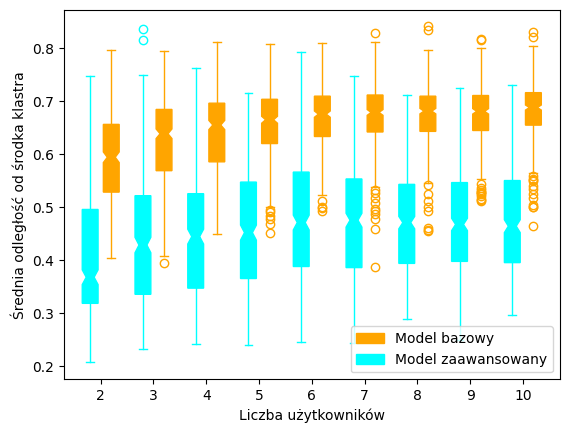
\includegraphics[width=0.5\linewidth]{image_2024-01-20_005257648.png}
    \caption{Średnia klasteryzacja rekomendacji w zależności od długości playlisty}
    \label{fig:enter-label}
\end{figure}

Średnia odległość od środka klastra rośnie wraz z liczbą użytkowników, co jest zgodne z oczekiwaniami. Proporcje między stopniem klasteryzacji w modelu bazowym i zaawansowanym są zachowane. 

\section{Mikroserwis}

Zaimplementowano mikroserwis udostępniający REST API pozwalające na generowanie rekomendacji za pomocą modeli. Mikroserwis zaimplementowany został za pomocą frameworku FastAPI i może być uruchomiony w kontenerze Dockera.

\subsection*{Uruchomienie}

Do uruchomienia mikroserwisu wymagane jest zainstalowanie narzędzia Docker, SDK Javy, oraz zależności:

\begin{verbatim}
cd src
poetry shell
pip install lightfm==1.17 --no-use-pep517
poetry install
\end{verbatim}

\subsubsection*{Trenowanie modelu}

Przed uruchomieniem mikroserwisu należy wytrenować i zserializować modele. W tym celu należy umieścić dane w katalogu \texttt{data/v4}, a następnie wywołać polecenia:

\begin{verbatim}
cd src
python3 create_models.py
\end{verbatim}

Modele zostaną zserializowane przez bibliotekę \texttt{pickle} i zapisane w katalogu \texttt{serialized}.

\subsubsection*{Uruchomienie serwisu}
\begin{verbatim}
docker build -t ium .
docker run -p 8081:8081 -v ${PWD}:/predictions ium
\end{verbatim}

\subsubsection*{Generowanie rekomendacji}


Mikroserwis obsługuje zapytania HTTP typu POST zawierające w sobie listę identyfikatorów użytkowników, dla których wygenerowana ma zostać playlista. Odpowiedzią na zapytanie jest lista utworów, w której każdy element zwiera identyfikator utworu, jego nazwę, oraz nazwę wykonawcy. Szczegółowe informacje na temat schematu zapytań, odpowiedzi, etc. dostępne są po uruchomieniu mikroserwisu pod adresem \texttt{localhost:8081/doc}.

Na potrzeby umożliwienia realizacji eksperymentu A/B przyjęto założenie, że w każdym zapytaniu można wyróżnić użytkownika, który uruchamia proces generowania playlisty - może to być na przykład użytkownik obecnie zalogowany w aplikacji. Wybór modelu w eksperymencie A/B odywa się na podstawie wartości modulo $2$ hasha identyfikatora użytkownika uruchamiającego generowanie playlisty.

Dostępne endpointy:
\begin{itemize}
\item POST \texttt{/predict} - generuje rekomendacje z bazowego lub zaawansowanego modelu na rzecz testu A/B. 
\item POST \texttt{/predict/base} - predykcja za pomocą modelu bazowego
\item POST \texttt{/predict/advanced} - predykcja za pomocą modelu zaawansowanego
\end{itemize}

Wszystkie rekomendacje wraz z dostarczonym wejściem i metadanymi będą zapisywane w wolumenie Dockera pod \texttt{/predictions/predictions.jsonl}.


\subsection*{Działanie}

Przykład uruchomienia modelu poza mikroserwisem dostępny jest w notatniku \texttt{example.ipynb}.

Generowanie predykcji (przebiega tak samo dla każdego z endpointów):

\begin{verbatim}
curl -X 'POST' \
  'http://localhost:8081/predict' \
  -H 'accept: application/json' \
  -H 'Content-Type: application/json' \
  -d '{
  "user_id": 123,
  "other_users": [
    124, 125, 126, 127, 128
  ],
  "playlist_length": 20
}'
\end{verbatim}

odpowiedź mikroserwisu:

\begin{verbatim}
[
  {
    "id": "2iUmqdfGZcHIhS3b9E9EWq",
    "name": "Everybody Talks",
    "artist": "Neon Trees"
  },
  {
    "id": "5FPnjikbwlDMULCCCa6ZCJ",
    "name": "Daughters",
    "artist": "John Mayer"
  },
  {
    "id": "3bXhtg6H8lOMWaLZttQF6F",
    "name": "Sunday Morning - Acoustic",
    "artist": "Maroon 5"
  },
  {
    "id": "0HRshWRNAwQBROvxXqG3i9",
    "name": "Skinny Love",
    "artist": "Birdy"
  },
<...>
]
\end{verbatim}

wpis w logu aplikacji (kolejno: eksperyment A/B, model zaawansowany, model bazowy):

\begin{verbatim}
DEBUG:    | 2024-01-19 21:46:22 | Model base/[ADVANCED] 20 songs
INFO:     172.17.0.1:60866 - "POST /predict HTTP/1.1" 200 OK
DEBUG:    | 2024-01-19 21:47:03 | Model ADVANCED        20 songs
INFO:     172.17.0.1:41046 - "POST /predict/advanced HTTP/1.1" 200 OK
DEBUG:    | 2024-01-19 21:48:47 | Model BASE    20 songs
INFO:     172.17.0.1:52470 - "POST /predict/base HTTP/1.1" 200 OK
\end{verbatim}

wygenerowany wpis w historii (\texttt{predictions.jsonl}):
\begin{verbatim}
{"user_id": 123, "other_users": [124, 125, 126, 127, 128], "playlist": 
["2iUmqdfGZcHIhS3b9E9EWq", "5FPnjikbwlDMULCCCa6ZCJ", "3bXhtg6H8lOMWaLZttQF6F", 
"0HRshWRNAwQBROvxXqG3i9", "3UH4JIDuP83866Y43bbo4k", "5rwdhliMmo0aAQ08vU0AOZ", 
"77Y57qRJBvkGCUw9qs0qMg", "2Xs64pHlU29DTVMjWKyblt", "7MRn6wgG0ReDRNYV5wJeGX", 
"1Kvbih7Ebm4bkPinpSottk", "6C88rHxXBlpcgtBY3HAF0E", "13HVjjWUZFaWilh2QUJKsP", 
"0RZyUsKfiC7MtiGKatCtGc", "5pbajJXEPdcoXQPXoAVR1t", "4gs07VlJST4bdxGbBsXVue", 
"3PSMcb1gU5A8DveqU2K4z2", "5WSdMcWTKRdN1QYVJHJWxz", "0tuyEYTaqLxE41yGHSsXjy", 
"2WwzQJt4hG7YC6x16ZTYFM", "562oeuAN5GH85iE7FQVKSB"], "timestamp": 
"2024-01-20 00:17:41.901890", "elapsed_time": 0.15295624732971191,
"model": "advanced", "is_ab": true}

\end{verbatim}


\end{document}
